\documentclass[UTF8,fontset=fandol]{ctexart}
\usepackage[margin=1.5cm]{geometry}
\usepackage{amsmath,amssymb}
\usepackage{enumitem}
\usepackage{tikz}
\usetikzlibrary{calc,arrows.meta,angles,quotes,patterns,positioning,decorations.pathreplacing,3d}
\usepackage{pgfplots}
\pgfplotsset{compat=1.18}

\newcommand{\sectionbanner}[2]{\section*{#1\quad #2}}
\newenvironment{question}[2]{\par\noindent\textbf{第#1题（#2分）}\par}{\par}
\newenvironment{choices}{\begin{enumerate}[label=\Alph*.,leftmargin=*]}{\end{enumerate}}
\newenvironment{multichoices}{\begin{enumerate}[label=\Alph*.,leftmargin=*]}{\end{enumerate}}
\newcommand{\choice}[1]{\item #1}
\newcommand{\subquestion}[2]{\par\noindent\textbf{（#1分）}#2\par}
\newcommand{\answerline}{\underline{\hspace{2cm}}}
\newcommand{\answerbox}[1]{\par\fbox{\rule{0pt}{#1}\hspace{0.9\linewidth}}\par}
\newenvironment{solution}[4]{%
  \par\noindent\textbf{第#1题\quad 答案：#2\quad 难度：#3\quad 知识点：#4}\par
}{\par}
\newcommand{\analysis}[1]{\par\textbf{思路分析：}#1\par}
\newcommand{\methodsummary}[1]{\par\textbf{方法总结：}#1\par}

\begin{document}
% UTF-8 LaTeX fragment: questions only

\sectionbanner{一、单选题}{共10题，每题5分，共50分}

\begin{question}{1}{5}
6年前，父亲的年龄是儿子的5倍；6年后，父亲的年龄是儿子的3倍。儿子今年多少岁？
\begin{choices}
  \choice{15}
  \choice{18}
  \choice{21}
  \choice{24}
\end{choices}
\end{question}

\begin{question}{2}{5}
有标着\(1,2,3,4,5,6\)的6张数字卡片。每次取两张不同的卡片，分别作为十位和个位，组成一个两位偶数。一共可以组成多少个不同的两位偶数？
\begin{choices}
  \choice{8}
  \choice{12}
  \choice{15}
  \choice{18}
\end{choices}
\end{question}

\begin{question}{3}{5}
在下图中，55个单位正方体被堆叠在一起。将这堆正方体的表面涂色，但与地面接触的底面不涂色。请问将这堆正方体拆开后，共有多少个完全未被涂色的单位正方体？

% Source figure: page-03.png
\begin{center}
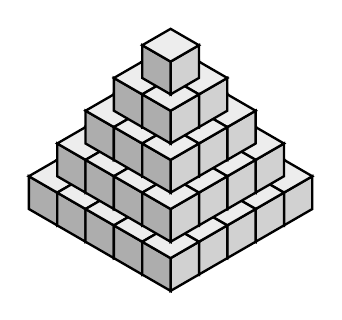
\begin{tikzpicture}[
  x={(0.36cm,-0.208cm)},
  y={(-0.36cm,-0.208cm)},
  z={(0cm,0.416cm)},
  line join=miter,
  line cap=butt
]
  \newcommand{\unitcube}[3]{%
    % Right face
    \filldraw[fill=black!18, draw=black, line width=0.85pt]
      (#1+1,#2,#3) -- (#1+1,#2+1,#3) --
      (#1+1,#2+1,#3+1) -- (#1+1,#2,#3+1) -- cycle;
    % Left face
    \filldraw[fill=black!32, draw=black, line width=0.85pt]
      (#1,#2+1,#3) -- (#1+1,#2+1,#3) --
      (#1+1,#2+1,#3+1) -- (#1,#2+1,#3+1) -- cycle;
    % Top face
    \filldraw[fill=black!7, draw=black, line width=0.85pt]
      (#1,#2,#3+1) -- (#1+1,#2,#3+1) --
      (#1+1,#2+1,#3+1) -- (#1,#2+1,#3+1) -- cycle;
  }
  % Back-to-front, bottom-to-top so outlines stay crisp.
  \foreach \k/\off/\n in {0/0/4, 1/0.5/3, 2/1/2, 3/1.5/1, 4/2/0} {
    \foreach \j in {0,...,\n} {
      \foreach \i in {0,...,\n} {
        \unitcube{\i+\off}{\j+\off}{\k}
      }
    }
  }
\end{tikzpicture}
\end{center}

\begin{choices}
  \choice{6}
  \choice{9}
  \choice{13}
  \choice{14}
  \choice{18}
\end{choices}
\end{question}

\begin{question}{4}{5}
小明从甲地到乙地，前一半路程的速度是每小时12千米，后一半路程的速度是每小时18千米。全程的平均速度是多少？
\begin{choices}
  \choice{每小时13.5千米}
  \choice{每小时14.4千米}
  \choice{每小时14千米}
  \choice{每小时15千米}
\end{choices}
\end{question}

\begin{question}{5}{5}
把下面7个图形作为一组，按原顺序不断重复排列：\(\bigcirc,\ \triangle,\ \triangle,\ \square,\ \star,\ \star,\ \square\)。从第1个图形开始计数，第2026个图形是哪个？
\begin{choices}
  \choice{\(\bigcirc\)}
  \choice{\(\star\)}
  \choice{\(\square\)}
  \choice{\(\triangle\)}
\end{choices}
\end{question}

\begin{question}{6}{5}
将4个边长均为\(5\text{ cm}\)且互不重叠的相同正方形，拼成了如下图所示的新图形。求这个新图形的周长。

% Source figure: page-06.png
\begin{center}
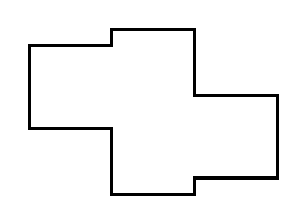
\begin{tikzpicture}[x=1.05cm,y=1.05cm,line width=1.1pt,line join=miter]
  \draw
    (0,0.8) -- (1,0.8) -- (1,1) -- (2,1) -- (2,0.2) --
    (3,0.2) -- (3,-0.8) -- (2,-0.8) -- (2,-1) --
    (1,-1) -- (1,-0.2) -- (0,-0.2) -- cycle;
\end{tikzpicture}
\end{center}

\begin{choices}
  \choice{15}
  \choice{20}
  \choice{30}
  \choice{45}
  \choice{50}
\end{choices}
\end{question}

\begin{question}{7}{5}
在\(1,2,3,\ldots,200\)中，正因数个数为偶数的数有多少个？
\begin{choices}
  \choice{14}
  \choice{180}
  \choice{186}
  \choice{196}
\end{choices}
\end{question}

\begin{question}{8}{5}
从\(1,2,3,\ldots,9\)中等可能地任取两个不同的数，这两个数的乘积是6的倍数的概率是多少？
\begin{choices}
  \choice{\(\dfrac{7}{36}\)}
  \choice{\(\dfrac{1}{3}\)}
  \choice{\(\dfrac{7}{18}\)}
  \choice{\(\dfrac{4}{9}\)}
\end{choices}
\end{question}

\enlargethispage{10mm}
\begin{question}{9}{5}
图中显示了一个带有三个障碍物的\(6\times6\)棋盘。一只蚂蚁在左上角，想要到达右下角。它只能在共用一条边的方格之间爬行，并且只能向下或向右爬行。它不能穿过任何障碍物。请问它共有多少条不同的路径可以走？

% Source figure: page-09.png
{\centering
\vspace{-1mm}
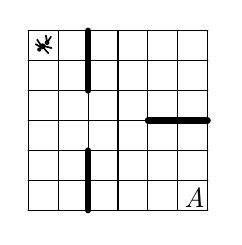
\begin{tikzpicture}[scale=0.38,line cap=round,line join=round]
  \draw[step=1cm,thin] (0,0) grid (6,6);
  % Three impassable barriers.
  \draw[line width=2.2pt] (2,4) -- (2,6);
  \draw[line width=2.2pt] (2,0) -- (2,2);
  \draw[line width=2.2pt] (4,3) -- (6,3);
  % A small vector ant in the upper-left cell.
  \fill (0.48,5.48) circle (0.10);
  \fill (0.63,5.60) circle (0.08);
  \fill (0.37,5.37) circle (0.07);
  \draw[line width=0.6pt]
    (0.43,5.44)--(0.25,5.55)
    (0.44,5.49)--(0.30,5.70)
    (0.52,5.42)--(0.67,5.25)
    (0.56,5.48)--(0.78,5.42)
    (0.67,5.66)--(0.76,5.80)
    (0.62,5.67)--(0.59,5.84);
  \node[font=\itshape] at (5.55,0.42) {A};
\end{tikzpicture}\par}

\begin{choices}
  \choice{88}
  \choice{90}
  \choice{92}
  \choice{96}
  \choice{112}
\end{choices}
\end{question}

\begin{question}{10}{5}
把正整数100写成两个或两个以上正整数之和。在所有写法中，各加数乘积的最大值是多少？
\begin{choices}
  \choice{\(2^{50}\)}
  \choice{\(5^{20}\)}
  \choice{\(2\times3^{33}\)}
  \choice{\(4\times3^{32}\)}
\end{choices}
\end{question}

\sectionbanner{二、填空题}{共5题，每题5分，共25分}

\begin{question}{11}{5}
袋中有3个红球和2个白球，除颜色外完全相同。从中不放回地随机取出2个球。将至少取到1个红球的概率化为最简分数后，分子与分母的和是\answerline
\end{question}

\begin{question}{12}{5}
\[
  1!+2!+3!+\cdots+2026!
\]
除以15的余数是\answerline
\end{question}

\Needspace{6.5cm}
\begin{question}{13}{5}
将四个相同的棋子放入如下图所示黑白相间的\(4\times4\)棋盘中。每个方格最多只能放置一个棋子。所有棋子必须放置在相同颜色的方格中，并且任意两个棋子不能处于同一行或同一列。请问共有多少种不同的放置方法？\answerline

% Source figure: page-13.png
\begin{center}
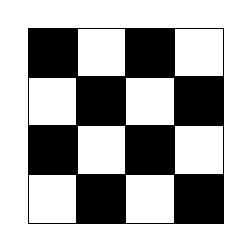
\begin{tikzpicture}[scale=0.62]
  \foreach \r in {0,...,3}{
    \foreach \c in {0,...,3}{
      \pgfmathtruncatemacro{\shadecell}{mod(\r+\c,2)}
      \ifnum\shadecell=0
        \fill[black] (\c,3-\r) rectangle ++(1,1);
      \else
        \fill[white] (\c,3-\r) rectangle ++(1,1);
      \fi
    }
  }
  \draw[step=1cm,thin] (0,0) grid (4,4);
\end{tikzpicture}
\end{center}
\end{question}

\begin{question}{14}{5}
不超过2026且与2026互质的正整数共有\answerline 个。
\end{question}

\begin{question}{15}{5}
参考下图，图中展示了一卷圆柱形的卷筒卫生纸，中间部分由空心纸板卷筒组成。卫生纸被分成若干节，卷在纸板上。包装上标明：“每节\(138\text{ mm}\times100\text{ mm}\)，3层”，这意味着每节长\(138\text{ mm}\)，宽\(100\text{ mm}\)，且包含3层。已知单层卫生纸的厚度为\(0.13\text{ mm}\)，纸板筒的直径为\(5\text{ cm}\)，整卷卫生纸的直径为\(12\text{ cm}\)，请问这一卷中大约有多少节卫生纸（结果四舍五入到整数）？（取\(\pi=3.14\)）

% Source figure: user-provided original — debugged in _q15fig.tex
\noindent
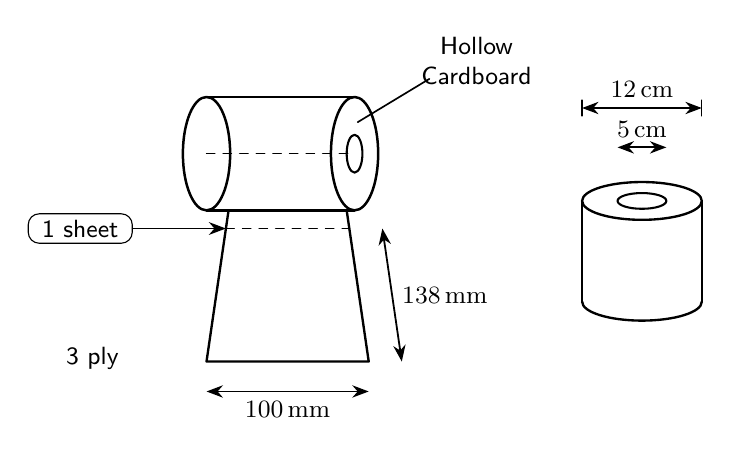
\begin{tikzpicture}[>=Stealth, line cap=round, line join=round, font=\sffamily\small]
  % ===== Left: 3-D horizontal roll =====
  \coordinate (R) at (2.20,3.55);
  \def\rx{0.30}
  \def\ry{0.72}
  \def\len{1.88}
  \coordinate (L) at ($(R)+(-\len,0)$);

  \fill[white]
    ($(L)+(0,-\ry)$) -- ($(R)+(0,-\ry)$)
    -- ($(R)+(0,\ry)$) -- ($(L)+(0,\ry)$) -- cycle;
  \draw[line width=0.9pt] ($(L)+(0,\ry)$) -- ($(R)+(0,\ry)$);
  \draw[line width=0.9pt] ($(L)+(0,-\ry)$) -- ($(R)+(0,-\ry)$);
  \filldraw[fill=white, draw=black, line width=0.9pt]
    (L) ellipse[x radius=\rx, y radius=\ry];
  \filldraw[fill=white, draw=black, line width=0.9pt]
    (R) ellipse[x radius=\rx, y radius=\ry];
  \filldraw[fill=white, draw=black, line width=0.75pt]
    (R) ellipse[x radius=0.10, y radius=0.24];
  \draw[dashed, line width=0.55pt] (L) -- (R);

  \node[align=center] (hc) at ($(R)+(1.55,1.18)$) {Hollow\\Cardboard};
  \draw[line width=0.6pt] ($(R)+(0.95,0.95)$) -- ($(R)+(0.04,0.40)$);

  % Mild trapezoid, dashed "1 sheet" line just under the roll
  \coordinate (STL) at ($(L)+(0.28,-\ry)$);
  \coordinate (STR) at ($(R)+(-0.10,-\ry)$);
  \coordinate (SBL) at ($(STL)+(-0.28,-1.92)$);
  \coordinate (SBR) at ($(STR)+(0.28,-1.92)$);
  \draw[line width=0.85pt] (STL) -- (SBL) -- (SBR) -- (STR);
  \coordinate (SDL) at ($(SBL)!0.88!(STL)$);
  \coordinate (SDR) at ($(SBR)!0.88!(STR)$);
  \draw[dashed, line width=0.55pt] (SDL) -- (SDR);

  \node[draw, rounded corners=4pt, inner xsep=5pt, inner ysep=2.2pt, fill=white] (onesheet)
    at ($(SDL)+(-1.85,0)$) {1 sheet};
  \draw[->, line width=0.7pt] (onesheet.east) -- (SDL);
  \node (threeply) at ($(SBL)+(-1.45,0.04)$) {3 ply};

  % 100 mm: width of the bottom edge
  \draw[<->, line width=0.65pt]
    ([yshift=-3.8mm]SBL) -- ([yshift=-3.8mm]SBR)
    node[midway, below] {\(100\,\mathrm{mm}\)};
  % 138 mm: from the dashed line DOWN to the bottom of the sheet
  \draw[<->, line width=0.65pt]
    ([xshift=4.2mm]SDR) -- ([xshift=4.2mm]SBR)
    node[midway, right] {\(138\,\mathrm{mm}\)};

  % ===== Right: upright roll =====
  \coordinate (U) at (5.85,2.95);
  \def\urx{0.76}
  \def\ury{0.24}
  \def\uh{1.28}
  \def\irx{0.31}

  \draw[line width=0.85pt] ($(U)+(-\urx,0)$) -- ($(U)+(-\urx,-\uh)$);
  \draw[line width=0.85pt] ($(U)+(\urx,0)$) -- ($(U)+(\urx,-\uh)$);
  \draw[line width=0.85pt]
    ($(U)+(-\urx,-\uh)$) arc[start angle=180,end angle=360,x radius=\urx,y radius=\ury];
  \filldraw[fill=white, draw=black, line width=0.85pt]
    (U) ellipse[x radius=\urx, y radius=\ury];
  \filldraw[fill=white, draw=black, line width=0.75pt]
    (U) ellipse[x radius=\irx, y radius=0.10];

  \draw[<->, line width=0.65pt]
    ($(U)+(-\urx,1.18)$) -- ($(U)+(\urx,1.18)$)
    node[midway, above] {\(12\,\mathrm{cm}\)};
  \draw[line width=0.5pt] ($(U)+(-\urx,1.08)$) -- ($(U)+(-\urx,1.28)$);
  \draw[line width=0.5pt] ($(U)+(\urx,1.08)$) -- ($(U)+(\urx,1.28)$);
  \draw[<->, line width=0.65pt]
    ($(U)+(-\irx,0.68)$) -- ($(U)+(\irx,0.68)$)
    node[midway, above] {\(5\,\mathrm{cm}\)};
\end{tikzpicture}

\end{question}

\sectionbanner{三、综合题}{共3题，每题15分，共45分}

\begin{question}{16}{15}
在3000多年前的古埃及，有一份著名的数学文献《莱因德数学纸草书》。考古学家发现，古埃及人对分数有一种奇特的“强迫症”——他们极其偏爱分子为1的分数（例如\(\frac12,\frac13,\frac14\)），我们现在称之为“古埃及分数”。在古埃及人的账本里，任何一个真分数，都必须拆分成几个“古埃及分数”相加的形式。为了完成这种拆分，古埃及大祭司们定下了两条极其严格的铁律：

铁律1：拆分出来的所有分数，分子必须全都是1。

铁律2：拆分出来的分数，分母绝对不能重复！（例如：把\(\frac35\)写成\(\frac15+\frac15+\frac15\)是犯法的，因为分母重复了！）

那么，古埃及人是怎么把\(\frac35\)这样分子不是1的分数拆开，又不违反规则的呢？聪明的大祭司发明了一个“魔法拆分公式”：他们发现，任何一个分子为1的分数，都可以裂变成两个更小的、且分母不同的古埃及分数。公式如下：
\[
  \frac1n=\frac1{n+1}+\frac1{n\times(n+1)}
\]
（注：\(n\)代表同一个非零自然数）

【魔法演示】假设我们要拆分\(\frac13\)（此时公式里的\(n=3\)）：
\[
  \frac13=\frac1{3+1}+\frac1{3\times(3+1)}
  =\frac14+\frac1{12}.
\]
你看！\(\frac13\)成功变成两个不同的古埃及分数相加，并且验证一下：
\[
  \frac14+\frac1{12}=\frac3{12}+\frac1{12}
  =\frac4{12}=\frac13,
\]
完全正确！

\subquestion{5}{古埃及法老要求把\(\frac34\)块黄金分给大臣。以下四位学者的拆分方案中，哪一个完全符合古埃及分数的“两条铁律”？}
\begin{choices}
  \choice{\(\dfrac34=\dfrac14+\dfrac14+\dfrac14\)}
  \choice{\(\dfrac34=\dfrac12+\dfrac14\)}
  \choice{\(\dfrac34=\dfrac24+\dfrac14\)}
  \choice{\(\dfrac34=\dfrac13+\dfrac13+\dfrac1{12}\)}
\end{choices}

\subquestion{5}{请你模仿材料中的“魔法拆分公式”，把\(\frac16\)拆分成两个不同的古埃及分数相加。}
\[
  \frac16=\frac1{(\quad)}+\frac1{(\quad)}
\]
（注意：请在括号内填入适当的纯数字，且要求第一个括号里的数字比第二个括号里的数字小）请问第二个括号里应该填写的数字是？
\answerspace

\subquestion{5}{前面提到，古埃及人不能把\(\frac25\)直接写成\(\frac15+\frac15\)。现在，请你利用刚才学到的所有知识，帮古埃及人把\(\frac25\)拆分成三个完全不同的古埃及分数相加。}
\[
  \frac25=\frac1{(\quad)}+\frac1{(\quad)}+\frac1{(\quad)}
\]
（提示：你可以先暂时把它写成\(\frac15+\frac15\)，然后对其中一个\(\frac15\)使用魔法拆分公式！请按照数字从小到大的顺序填写分母）请问最后一个空应该填写几？
\answerspace
\end{question}

\begin{question}{17}{15}
如图1所示，考虑在边长为\(1\text{ cm}\)的正六边形\(ABCDEF\)内部沿直线运动的点\(P\)的轨迹。当点\(P\)到达边界（边）时，会如图2所示发生反弹（注：入射角等于反射角）。但是，若点\(P\)恰好到达正六边形的顶点，则会在该顶点处停止运动。现已知点\(P\)从顶点\(A\)出发，且其轨迹的第一次反弹发生在边\(CD\)上的某一点。请回答下列问题。请根据上述规则回答以下问题：

% Source figures: page-19.png
\begin{center}
\begin{tikzpicture}[>=Stealth,line cap=round,line join=round]
  \begin{scope}[xshift=-3.2cm,scale=1.55]
    \coordinate (A) at (0,1);
    \coordinate (B) at (-0.866,0.5);
    \coordinate (C) at (-0.866,-0.5);
    \coordinate (D) at (0,-1);
    \coordinate (E) at (0.866,-0.5);
    \coordinate (F) at (0.866,0.5);
    \coordinate (X) at (-0.30,-0.827);
    \coordinate (P) at (0.03,-0.52);
    \draw (A)--(B)--(C)--(D)--(E)--(F)--cycle;
    \draw (A)--(X);
    \draw[->] (X)--(P);
    \node[above] at (A) {\(A\)};
    \node[left] at (B) {\(B\)};
    \node[left] at (C) {\(C\)};
    \node[below] at (D) {\(D\)};
    \node[right] at (E) {\(E\)};
    \node[right] at (F) {\(F\)};
    \node[above right] at (P) {\(P\)};
    \node at (0,-1.45) {图1};
  \end{scope}

  \begin{scope}[xshift=2.3cm,yshift=-0.35cm]
    \node[align=center] at (0,2.25) {使做了标记的两个角大小相等地反弹。};
    \draw (-1.65,0)--(1.65,0);
    \draw (-1.50,1.80)--(0,0);
    \draw[->] (0,0)--(0.78,1.02);
    \draw (0,0) ++(180:0.43)
      arc[start angle=180,end angle=130,radius=0.43];
    \draw (0,0) ++(0:0.43)
      arc[start angle=0,end angle=53,radius=0.43];
    \node at (0,-0.48) {图2};
  \end{scope}
\end{tikzpicture}
\end{center}

\subquestion{5}{在边\(CD\)上完成第一次反弹后，点\(P\)接下来可能到达的边有哪些？}
\begin{choices}
  \choice{边\(AB\)和边\(BC\)}
  \choice{边\(BC\)和边\(DE\)}
  \choice{边\(AF\)和边\(EF\)}
  \choice{边\(AB\)和边\(AF\)}
\end{choices}

\subquestion{5}{若点\(P\)首先在边\(CD\)上的点\(X\)处发生反弹，在接下来到达的边上又发生了1次反弹（共反弹2次），最终恰好到达了顶点\(D\)。求线段\(CX\)的长度。}
\begin{choices}
  \choice{\(\dfrac14\text{ cm}\)}
  \choice{\(\dfrac13\text{ cm}\)}
  \choice{\(\dfrac12\text{ cm}\)}
  \choice{\(\dfrac23\text{ cm}\)}
\end{choices}

\subquestion{5}{若点\(P\)首先在边\(CD\)上的点\(Y\)处发生反弹，接着又连续发生了2次反弹（共反弹3次），最终恰好到达了顶点\(D\)。求线段\(CY\)的长度。}
\begin{choices}
  \choice{\(\dfrac35\text{ cm}\)}
  \choice{\(\dfrac47\text{ cm}\)}
  \choice{\(\dfrac57\text{ cm}\)}
  \choice{\(\dfrac58\text{ cm}\)}
\end{choices}
\end{question}

\begin{question}{18}{15}
袋子里装有写着数字1、2、3的卡片各若干张。每次从袋子中随机抽取1张卡片，确认上面的数字后，再将卡片放回袋中。按照抽出卡片上的数字，在方格地图上前进相应的步数。从“起点”出发，重复此抽卡前进的操作，请回答以下问题：

\subquestion{5}{若终点设定为第4格，恰好停在第4格的走法共有多少种？（\quad）}
\begin{choices}
  \choice{4}
  \choice{6}
  \choice{7}
  \choice{8}
\end{choices}

\subquestion{5}{若终点设定为图中的第10格，恰好停在第10格的走法共有多少种？（仅填写数字）}
\answerspace

\subquestion{5}{在第2问（走到第10格）的所有走法中，要求中途必须恰好停在第6格，符合条件的走法共有多少种？（仅填写数字）}
\answerspace
\end{question}

\clearpage
% UTF-8 LaTeX fragment: reference answers and solutions

\sectionbanner{一、单选题}{参考答案与解析}

\begin{solution}{1}{B}{4.0}{代数与方程应用}
\analysis{把两个时刻的倍数关系同时写出，利用父子年龄差始终不变统一比较。}
\begin{enumerate}[label=\textbf{Step \arabic*:},leftmargin=*]
  \item 设儿子今年\(x\)岁，父亲今年\(y\)岁。由题意
  \[
    y-6=5(x-6),\qquad y+6=3(x+6).
  \]
  \item 两式分别化为\(y=5x-24\)与\(y=3x+12\)，所以\(2x=36\)，得\(x=18\)。
  \item 回代得父亲今年66岁。6年前为\(60=5\times12\)，6年后为\(72=3\times24\)，条件都满足。因此选B。
\end{enumerate}
\methodsummary{把跨时刻条件转成同一时刻的等式，再用不变量消元。}
\end{solution}

\begin{solution}{2}{C}{6.0}{排列组合与概率}
\analysis{按个位是否为偶数分类，再用乘法原理计数。}
\begin{enumerate}[label=\textbf{Step \arabic*:},leftmargin=*]
  \item 两位数为偶数，个位只能从\(2,4,6\)中选，有3种。
  \item 个位确定后，十位可从剩余5张卡片中任选，有5种。
  \item 不同两位数共有\(3\times5=15\)个，因此选C。
\end{enumerate}
\methodsummary{先固定受限制的位置，再安排其余位置。}
\end{solution}

\begin{solution}{3}{D}{4.0}{几何与空间}
\analysis{采用“分层剥洋葱”法。因为底面不涂色，每一层未涂色的正方体都隐藏在几何体中心。将三维立体图形逐层拆解为二维平面正方形，减去暴露在外的最外圈，剩下的即为目标数量。}

我们把这堆正方体从上往下分成5层，每层从俯视图来看，都是一个实心的正方形阵列。因为四周都暴露在外面被涂色了，我们要把每一层最外围的一圈“剥掉”。一个正方形去掉外围一圈后，它的边长左右各减去1，上下各减去1，也就是边长总共减少了2。

从上往下逐层计算内部核心未被涂色的区域：第1层全部暴露被涂色，未涂色0个；第2层全部暴露被涂色，未涂色0个；第3层边长为3，去掉外圈，内部剩下
\[
  (3-2)\times(3-2)=1
\]
个；第4层边长为4，去掉外圈，内部剩下
\[
  (4-2)\times(4-2)=4
\]
个；第5层（最底层）边长为5，四周外圈被涂色，但“底面不涂色”保护了底部。去掉外圈，剩下内部是
\[
  (5-2)\times(5-2)=9
\]
个。最后，将各层未涂色的正方体数量相加：
\[
  0+0+1+4+9=14.
\]
因此，完全未被涂色的单位正方体共有14个，正确答案选择D。

\methodsummary{寻找未涂色方块只需采用“剥洋葱法”：剥去每一层暴露在外的一圈，各层内部隐藏的方块数量即为该层原边长减2的平方，即\((n-2)^2\)，将其逐层相加即可得出总数。}
\end{solution}

\begin{solution}{4}{B}{6.0}{代数与方程应用}
\analysis{平均速度必须用总路程除以总时间，等路程两段应使用调和式而非速度算术平均。}
\begin{enumerate}[label=\textbf{Step \arabic*:},leftmargin=*]
  \item 设前后两段路程都为36千米。两段用时分别为\(36\div12=3\)小时和\(36\div18=2\)小时。
  \item 总路程为72千米，总时间为5小时。
  \item 平均速度为\(72\div5=14.4\)千米/小时，因此选B。
\end{enumerate}
\methodsummary{平均速度只由总路程与总时间决定。}
\end{solution}

\begin{solution}{5}{D}{6.0}{新定义与抽象建模}
\analysis{把7个图形看作一个周期，用序号除以周期长度后的余数定位。}
\begin{enumerate}[label=\textbf{Step \arabic*:},leftmargin=*]
  \item 图形每7个重复一次。
  \item \(2026=7\times289+3\)，所以第2026个图形与每组中的第3个相同。
  \item 每组第3个图形是\(\triangle\)，因此选D。
\end{enumerate}
\methodsummary{周期题先求余数，余数为0时才对应周期末位。}
\end{solution}

\begin{solution}{6}{E}{4.0}{几何与空间}
\analysis{利用线段平移，将内凹边向外推，把不规则图形的周长转化为最小外接矩形周长。}

题目图形由4个边长为\(5\text{ cm}\)的正方形组成。对于这类不规则的多边形，最简便的方法是使用“线段平移法”：将所有内凹的线段（横向的向两端推，纵向的向上下推）平移到外侧。这样，原图形的周长就完全等于完全覆盖它的最小外接长方形的周长。

该图形可以被切割为左、中、右三个区域。其中左侧和右侧各由1个正方形覆盖，中间区域由2个正方形竖直覆盖。宽度（横向）整体横跨了3个正方形的宽度，所以宽为
\[
  5\times3=15\text{ cm}.
\]
高度（纵向）中间区域上下堆叠了2个正方形，所以高为
\[
  5\times2=10\text{ cm}.
\]
根据长方形周长公式，代入数据得
\[
  (15+10)\times2=50\text{ cm}.
\]
因此，这个新图形的周长是\(50\text{ cm}\)，正确答案选E。

\methodsummary{利用“线段平移法”，将图形所有凹陷的边缘向外平移，不规则图形的周长问题即可转化为求其最小外接矩形的周长。}
\end{solution}

\begin{solution}{7}{C}{8.0}{数论与整除逻辑}
\analysis{正因数通常成对出现，只有完全平方数的平方根会与自身配对。}
\begin{enumerate}[label=\textbf{Step \arabic*:},leftmargin=*]
  \item 若\(m\)不是完全平方数，每个因数\(d\)都与不同的因数\(m/d\)配对，因数个数为偶数。完全平方数恰有一个自配对因数，因数个数为奇数。
  \item 不超过200的完全平方数为\(1^2,2^2,\ldots,14^2\)，共14个，因为
  \[
    14^2=196<200<225=15^2.
  \]
  \item 所求个数为\(200-14=186\)，选C。
\end{enumerate}
\methodsummary{因数配对把因数奇偶问题转成平方数计数。}
\end{solution}

\begin{solution}{8}{C}{8.0}{排列组合与概率}
\analysis{按无序数对计数，用整除条件分类或补集压缩，最后除以36个总数对。}

总的无序数对数量为
\[
  \binom92=36.
\]
乘积为6的倍数的数对为
\[
\begin{gathered}
  (1,6),(2,3),(2,6),(2,9),(3,4),(3,6),(3,8),\\
  (4,6),(4,9),(5,6),(6,7),(6,8),(6,9),(8,9),
\end{gathered}
\]
共14对。因而概率为
\[
  \frac{14}{36}=\frac7{18}.
\]
所以选C。

\methodsummary{概率计数必须让分子分母使用同一种有序或无序口径。}
\end{solution}

\begin{solution}{9}{A}{6.0}{几何与空间}
\analysis{利用“标数法”（加法原理）解题。网格中任一无障碍格子的路径数，等于到达它上方格子的路径数与左方格子的路径数之和。遇到不可穿透的障碍墙，则该方向传导的路径数视为0。}

\begin{enumerate}[label=\textbf{Step \arabic*:},leftmargin=*]
  \item \textbf{锁定唯一“关卡”。}列号单调不减，从“第2列跨到第3列”这件事在一条路径中只发生一次，记该步所在行为过闸行。墙①封第1、2行，墙②封第5、6行，故过闸行属于第3、4行。于是全局问题化为“按过闸行分类”的两类互斥且穷尽的情形。

  \item \textbf{情况一前置：过闸前（第3行过闸）。}过闸前活动域被墙①限制为左两列、上三行的\(3\times2\)小块，从\((1,1)\)走到\((3,2)\)需\(2\mathrm D+1\mathrm R\)：
  \[
    N_1^{\text{前}}=\binom31=3.
  \]

  \item \textbf{情况一后置：过闸后（扣除撞墙③者）。}过闸后在\((3,3)\)，到\((6,6)\)需\(3\mathrm D+3\mathrm R\)，不受墙限制时共
  \[
    \binom63=20.
  \]
  其中撞墙③的路径必在第3行先到达第5列（墙③在第3、4行之间的第5、6列）。从\((3,3)\)到\((3,5)\)只有\(2\mathrm R\)一种走法；再由\((3,5)\)到\((6,6)\)需\(3\mathrm D+1\mathrm R\)，共
  \[
    \binom41=4
  \]
  条，且这4条均无法下穿墙③。故合法后置数为
  \[
    N_1^{\text{后}}=\binom63-\binom41=20-4=16.
  \]

  \item \textbf{情况一总数（乘法原理）。}过闸前、后两段独立，
  \[
    N_1=N_1^{\text{前}}\times N_1^{\text{后}}=3\times16=48.
  \]

  \item \textbf{情况二前置：过闸前（第4行过闸）。}过闸前在左两列、上四行，从\((1,1)\)走到\((4,2)\)需\(3\mathrm D+1\mathrm R\)：
  \[
    N_2^{\text{前}}=\binom41=4.
  \]

  \item \textbf{情况二后置：过闸后（墙③已无关）。}过闸后已在\((4,3)\)，墙③位于第3、4行之间，已处于其下方，不可能再被挡。从\((4,3)\)到\((6,6)\)需\(2\mathrm D+3\mathrm R\)：
  \[
    N_2^{\text{后}}=\binom52=10.
  \]
  所以\(N_2=4\times10=40\)。

  \item \textbf{总数（加法原理）。}两类互斥且穷尽：
  \[
    N=N_1+N_2=48+40=\boxed{88}.
  \]
\end{enumerate}

\methodsummary{利用“标数法”（加法原理），每个格子的可达路径数等于它上方和左方相邻格子路径数之和，遇到障碍边界则对应的路径数不计入，逐格推导至终点即可。}
\end{solution}

\begin{solution}{10}{D}{8.0}{代数与方程应用}
\analysis{用局部替换证明加数只能取2或3，且三个2应改成两个3，最终按100除以3的余数构造。}

若全部加数均为1，则把其中两个1合并为2，可使乘积由1增至2，所以这种写法不可能最优。若有加数1和另一个加数\(m\ge2\)，把它们合成\(m+1\)会使乘积从\(m\)增到\(m+1\)，所以其他含1的写法也不可能最优。因此最优写法中没有加数1。

若有加数\(m\ge5\)，将其换成3与\(m-3\)，新乘积为
\[
  3(m-3)>m,
\]
所以最优写法只需2、3、4，而4可看成\(2+2\)。

三个2的乘积8小于两个3的乘积9，所以2最多出现两个。因为
\[
  100=3\times32+4,
\]
最优写法为32个3和两个2，最大乘积为
\[
  4\times3^{32}.
\]
故选D。

\methodsummary{整数和的最大乘积要用局部增益替换证明结构，再给出可达构造。}
\end{solution}

\sectionbanner{二、填空题}{参考答案与解析}

\begin{solution}{11}{19}{6.0}{排列组合与概率}
\analysis{“至少一个红球”的补事件是“两球全白”，先用补集求出概率，再按题意取最简分数的分子与分母之和。}
\begin{enumerate}[label=\textbf{Step \arabic*:},leftmargin=*]
  \item 从5个球中取2个，等可能组合总数为
  \[
    \binom52=10.
  \]
  \item 两球全白的组合数为
  \[
    \binom22=1.
  \]
  \item 至少取到1个红球的概率为
  \[
    1-\frac1{10}=\frac9{10}.
  \]
  \item 上一步所得分数已经是最简分数，所以分子与分母的和为
  \[
    9+10=19.
  \]
\end{enumerate}
\methodsummary{“至少”事件优先检查补集是否更短；求出概率后要继续完成题目指定的分数运算。}
\end{solution}

\begin{solution}{12}{3}{8.0}{数论与整除逻辑}
\analysis{从\(5!\)开始每个阶乘都含因子15，后面整段对余数没有贡献。}
\begin{enumerate}[label=\textbf{Step \arabic*:},leftmargin=*]
  \item 对任意\(m\ge5\)，\(m!\)含有因子\(3\times5=15\)，所以\(m!\)除以15余数为0。
  \item 原和与前四项之和同余：
  \[
    1!+2!+3!+4!=1+2+6+24=33.
  \]
  \item 33除以15的余数为3。
\end{enumerate}
\methodsummary{模合数时可寻找阶乘中各质因子首次齐全的位置。}
\end{solution}

\begin{solution}{13}{8}{6.0}{几何与空间}
\analysis{采用分类与分步结合的策略。首先按颜色分类（全黑或全白）。其次在同色方格中分步放置：由于不能同行同列，第一、三行的落子会相互限制，第二、四行也会独立相互限制，分别计算后再相乘。}

这是一个带有颜色和位置双重限制的排列组合问题。四个棋子颜色一致，即全在黑格或全在白格；任意两个棋子不能在同一行，也不能在同一列。

\begin{enumerate}[label=\textbf{Step \arabic*:},leftmargin=*]
  \item 先假设所有棋子都放在黑色方格中。第1行有2个黑格可供放置。一旦第1行的黑格被选中，为了满足“不同列”的要求，第3行放置棋子时，就只能选择剩下的那1个与第1行不同列的黑格。因此，在第1行和第3行放置棋子共有\(2\times1=2\)种方法。
  \item 同理，第2行的黑格与第1、3行的黑格天然不在同一列，互不干扰。第2行也有2个黑格可选；选定后，第4行只剩1个符合条件的黑格。因此，在第2行和第4行放置棋子也有\(2\times1=2\)种方法。
  \item 根据乘法原理，所有棋子都放在黑色方格中的总方法数为\(2\times2=4\)种。
  \item 黑白方格在棋盘上的分布完全对称，将所有棋子放在白色方格中同样有4种方法。根据加法原理，总方法数为
  \[
    4+4=8.
  \]
\end{enumerate}

\methodsummary{利用“分类讨论结合乘法原理”，先按黑白颜色分类，再分别计算奇偶行（或列）互不干扰的放置方法数并相乘，最后将两类结果相加即可。}
\end{solution}

\begin{solution}{14}{1012}{8.0}{数论与整除逻辑}
\analysis{分解\(2026=2\times1013\)，在1到2026中排除2或1013的倍数。}

因为
\[
  2026=2\times1013,
\]
又有
\[
  \sqrt{1013}<32.
\]
逐一试除不超过31的质数\(3,5,7,11,13,17,19,23,29,31\)，均不能整除1013，所以1013是质数。因此，与2026不互质的数恰为2的倍数或1013的倍数。

不超过2026的偶数有1013个，1013的倍数有2个，同时为二者倍数的只有2026一个。因此不互质的数有
\[
  1013+2-1=1014
\]
个。所求为
\[
  2026-1014=1012.
\]

\methodsummary{互质计数先找全部不同质因数，再对其倍数集合做容斥。}
\end{solution}

\begin{solution}{15}{174}{6.0}{几何与空间}
\analysis{本题的核心解题逻辑是体积守恒。整卷卫生纸（纯纸张部分）的体积，必定等于所有单节卫生纸展开后的长方体总体积。统一量纲：题目中交替使用\(\text{cm}\)和\(\text{mm}\)，解题第一步必须统一单位（建议统一转化为\(\text{cm}\)）。计算总体积：利用圆柱体体积公式，计算外圆柱与内部空心纸板筒的体积差，得出纯纸张的总体积。计算单节体积：将单节卫生纸看作一个薄长方体，其体积等于长\(\times\)宽\(\times\)（单层厚度\(\times\)层数）。计算总数量：用总体积除以单节纸张的体积，得到总节数，最后根据题意进行四舍五入取整。}

\begin{enumerate}[label=\textbf{Step \arabic*:},leftmargin=*]
  \item 圆柱体的体积由底面积乘以高求得。首先，统一单位为厘米：卫生纸的高度为
  \[
    100\text{ mm}=10\text{ cm}.
  \]
  整卷卫生纸的外径为\(12\text{ cm}\)，内部空心纸板筒的直径为\(5\text{ cm}\)。因此，1卷卫生纸（纯纸张部分）的体积为
  \[
    3.14\times\left(\frac{12}{2}\right)^2\times10
    -3.14\times\left(\frac{5}{2}\right)^2\times10
    =934.15\text{ cm}^3.
  \]

  \item 将单节的长和厚度转换为厘米：
  \[
    138\text{ mm}=13.8\text{ cm},\qquad
    0.13\text{ mm}=0.013\text{ cm}.
  \]
  因为每节卫生纸有3层，所以每一节的体积为
  \[
    10\times13.8\times0.013\times3=5.382\text{ cm}^3.
  \]

  \item 将总纸张体积除以单节体积：
  \[
    \frac{934.15}{5.382}\approx173.57.
  \]
  根据题目要求四舍五入到整数，即为174节。
\end{enumerate}

\methodsummary{把握“体积守恒”核心，在统一单位的前提下，用空心圆柱纸张的总净体积除以单节展开后的长方体体积，即可求出总节数。}
\end{solution}

\sectionbanner{三、综合题}{参考答案与解析}

\begin{solution}{16（1）}{B}{4.0}{新定义与抽象建模}
\analysis{紧扣古埃及分数的“两条铁律”进行排查。铁律1要求分子必须全为1；铁律2要求分母绝对不能重复。只需逐一检验选项是否违规即可得出唯一正确答案。}

A选项：
\[
  \frac34=\frac14+\frac14+\frac14,
\]
分母重复了三个4，违反铁律2，排除。

B选项：
\[
  \frac34=\frac12+\frac14,
\]
分子全为1，分母分别是2和4，没有重复，完全符合两条铁律，正确。

C选项：
\[
  \frac34=\frac24+\frac14,
\]
其中\(\frac24\)分子不是1，违反铁律1，排除。

D选项：
\[
  \frac34=\frac13+\frac13+\frac1{12},
\]
分母重复了两个3，违反铁律2，排除。

\methodsummary{严格对照“分子必须为1且分母不重复”的两条新定义铁律，逐一“排雷”筛选选项。}
\end{solution}

\begin{solution}{16（2）}{42}{6.0}{新定义与抽象建模}
\analysis{第一个空填7；第二个空填42。这是对“魔法拆分公式”的直接运用。明确公式里的变量\(n=6\)，代入公式计算出两个新分母即可，注意题目要求数字按从小到大填空。}

已知魔法拆分公式：
\[
  \frac1n=\frac1{n+1}+\frac1{n\times(n+1)}.
\]
题目要拆分\(\frac16\)，令\(n=6\)。代入公式得分母分别为
\[
  6+1=7,\qquad 6\times7=42.
\]
根据题目要求“第一个比第二个小”，所以两空分别填7和42，第二个括号里填写42。

\methodsummary{运用“代入法”，将具体数字直接替换公式中的字母\(n\)，按运算顺序精准计算出新分母。}
\end{solution}

\begin{solution}{16（3）}{30}{6.0}{新定义与抽象建模}
\analysis{三个空依次填入5、6、30。核心策略是“先分后变”。先强行拆成两个\(\frac15\)相加，再利用公式对其中一个\(\frac15\)进行变身，最后按数字从小到大排序填空。}

\begin{enumerate}[label=\textbf{Step \arabic*:},leftmargin=*]
  \item 先强行拆分：
  \[
    \frac25=\frac15+\frac15.
  \]
  此时分母重复。
  \item 保留第一个\(\frac15\)不动，对第二个使用公式（令\(n=5\)），得
  \[
    \frac15=\frac16+\frac1{30}.
  \]
  \item 合并替换得
  \[
    \frac25=\frac15+\frac16+\frac1{30}.
  \]
  按从小到大顺序，分母依次为5、6、30。
\end{enumerate}

\methodsummary{采用“先分后变”的转化策略，先同分母强行拆分，再套用公式对局部进行等量替换。}
\end{solution}

\begin{solution}{17（1）}{C}{4.0}{新定义与抽象建模}
\analysis{将边\(CD\)视为透明窗户，利用镜面反射原理。寻找起点\(A\)关于\(CD\)的镜像对称点\(A'\)，把反弹轨迹等效为从\(A'\)发出的直射光束，扫射边界即可。}

找镜像点：在正六边形中，对角线\(AC\)与边\(CD\)恰好垂直，因为
\[
  120^\circ-30^\circ=90^\circ.
\]
若把\(CD\)当作镜面向下翻折，\(A\)的镜像点\(A'\)正好位于\(A\)到\(C\)连线的延长线上。

光束扫射：从\(A'\)点向“窗户”\(CD\)打出光束。当光线擦着极左端\(C\)点射出时，沿直线\(A'C\)会笔直命中顶点\(A\)。当光线擦着极右端\(D\)点射出时，沿直线\(A'D\)连线延长，恰好精准命中顶点\(E\)。

反弹后的光束呈扇形，其辐射范围被严密限制在顶点\(A\)到顶点\(E\)之间。因此，这束光只能打在正六边形右侧的边\(AF\)和边\(EF\)上。

\methodsummary{遇到折线反射，把反射面当透明窗户，从起点的“镜像分身”拉直连线，寻找光束两端的极值边界。}
\end{solution}

\begin{solution}{17（2）}{B}{6.0}{新定义与抽象建模}
\analysis{2次反弹相当于跨越2层镜像。将终点\(D\)往下翻折两次得到终极目标\(D_2\)。连接起点\(A\)与\(D_2\)，形成拉直的轨迹，利用相似三角形的比例求解。}

\begin{enumerate}[label=\textbf{Step \arabic*:},leftmargin=*]
  \item \textbf{建构楼层。}设正六边形的平行对边间距为1个“楼层高”。起点\(A\)位于第一面镜子\(CD\)上方1层。
  \item \textbf{定位终点。}终点\(D\)经过2次镜像翻折（向下延展），其最终的镜像点\(D_2\)位于\(CD\)镜面下方2层的位置。
  \item \textbf{拉直连线。}将真实的曲折轨迹拉直为直线\(AD_2\)，该直线穿过\(CD\)边交于点\(X\)。
  \item \textbf{比例分配。}直线在垂直方向上的落差比为\(1:2\)（上方1层、下方2层）。根据相似三角形等比例放大原理，它在水平方向上分得的距离比例也为\(1:2\)。
  \item \textbf{计算结果。}边\(CD\)的总长度为\(1\text{ cm}\)，因此\(CX\)占水平总长度的
  \[
    \frac1{1+2},
  \]
  即
  \[
    CX=\frac13\text{ cm}.
  \]
\end{enumerate}

\methodsummary{将多次反弹转化为多层镜面翻折，连接起点与最终镜像点，用“垂直楼层数之比＝水平路程之比”求解。}
\end{solution}

\begin{solution}{17（3）}{C}{6.0}{新定义与抽象建模}
\analysis{3次反弹需翻折3层找到目标\(D_3\)。在密铺网格中精准数出\(D_3\)的“水平总位移”和“垂直总落差”，再次利用相似三角形的比例分配求解。}

\begin{enumerate}[label=\textbf{Step \arabic*:},leftmargin=*]
  \item \textbf{寻找第三层终点。}经过3次镜面翻折，终点\(D\)被映射到了更远更深的第3层镜像点\(D_3\)。
  \item \textbf{测算总跨度。}借助六边形密铺网格观察，目标\(D_3\)相对于参考点\(C\)，在水平方向上向右偏移了2.5个边长，即水平总宽度为\(2.5\text{ cm}\)。
  \item \textbf{测算总落差。}在垂直方向上，起点\(A\)在\(CD\)上方1层，而\(D_3\)位于\(CD\)下方2.5层，因此总垂直落差为
  \[
    1+2.5=3.5
  \]
  层。
  \item \textbf{相似比例。}直线\(AD_3\)穿过\(CD\)边交于点\(Y\)。直线在通过第一面镜子前，走过的垂直比例是
  \[
    \frac1{3.5}=\frac27.
  \]
  \item \textbf{计算结果。}水平方向的路程\(CY\)也占总水平宽度的\(\frac27\)，即
  \[
    CY=2.5\times\frac27=\frac57\text{ cm}.
  \]
\end{enumerate}

\methodsummary{无论反弹多少次，核心就是锁定最终镜像点的“总水平宽度”和“总垂直落差”，用单一比例算式求解截距。}
\end{solution}

\begin{solution}{18（1）}{C}{4.0}{新定义与抽象建模}
\analysis{到达某格的走法数，等于到达它前面一、二、三格的走法数之和。依次写出前几个格子的走法即可求出。}

设到达第\(n\)格的走法为\(W(n)\)。
\begin{enumerate}[label=\textbf{Step \arabic*:},leftmargin=*]
  \item 走1步到第1格，只有走1一种，即\(W(1)=1\)。
  \item 到第2格，可走\(1+1\)或直接跨2，即\(W(2)=2\)。
  \item 到第3格，可从起点跨3，或从第1、第2格跨来，即
  \[
    W(3)=1+1+2=4.
  \]
  \item 到第4格，只能从第1、2、3格跨来，故
  \[
    W(4)=W(1)+W(2)+W(3)=1+2+4=7.
  \]
\end{enumerate}
故有7种走法。

\methodsummary{运用递推法（或动态规划思想），提炼出状态转移方程，即“到达当前格的走法数等于到达它前面三格的走法数之和”，并穷举出前三格的初始基础走法。}
\end{solution}

\begin{solution}{18（2）}{274}{6.0}{新定义与抽象建模}
\analysis{基于第1问的递推关系，连续将前三项的数值相加得到下一项，一步步向后推导直至第10项。}

由上问知核心递推公式为
\[
  W(n)=W(n-1)+W(n-2)+W(n-3).
\]
已知前四项为
\[
  W(1)=1,\quad W(2)=2,\quad W(3)=4,\quad W(4)=7.
\]
依次推导后序项：
\[
\begin{aligned}
  W(5)&=2+4+7=13,\\
  W(6)&=4+7+13=24,\\
  W(7)&=7+13+24=44,\\
  W(8)&=13+24+44=81,\\
  W(9)&=24+44+81=149,\\
  W(10)&=44+81+149=274.
\end{aligned}
\]
所以，到达第10格共有274种走法。

\methodsummary{运用递推法（或动态规划思想），提炼出状态转移方程，即“到达当前格的走法数等于到达它前面三格的走法数之和”，并穷举出前三格的初始基础走法。}
\end{solution}

\begin{solution}{18（3）}{168}{6.0}{新定义与抽象建模}
\analysis{将路线拆分为“起点到第6格”和“第6格到第10格”两段独立的子路径。算出各自走法数后相乘。}

\begin{enumerate}[label=\textbf{Step \arabic*:},leftmargin=*]
  \item 第一阶段，从起点走到第6格。根据上问推导的递推结果，走法有\(W(6)=24\)种。
  \item 第二阶段，从第6格走到第10格。这段路程的跨度为
  \[
    10-6=4
  \]
  格，这与从起点出发走4格完全等价，走法有\(W(4)=7\)种。
  \item 由于这两个阶段连续发生且相互独立，根据分步乘法原理，总走法数为
  \[
    W(6)\times W(4)=24\times7=168.
  \]
\end{enumerate}
故共有168种符合条件的走法。

\methodsummary{运用分步乘法原理。将整个运动轨迹在“第6格”处切断，拆分为两个独立阶段。先求出从起点到达第6格的走法数，再求出从第6格到达第10格（相当于从头走4格）的走法数，最后将两个阶段的结果相乘即可。}
\end{solution}

\end{document}
